\documentclass[9pt]{beamer}

\usepackage[utf8x]{inputenc}
\usepackage[english]{babel}
\usepackage{amsmath, amsfonts, amssymb}
\usepackage{color}
\usepackage{xcolor}
\usepackage{tikz}
\usetikzlibrary{positioning,shapes,shadows,arrows,snakes}
\usepackage{listliketab}
\usepackage{shuffle}
\usepackage{xargs}
\usepackage{multirow}
\usepackage{pgfplots}
\usepackage{csquotes}
\usepackage{verbatim}

\definecolor{BlueGreen}{cmyk}{0.85,0,0.33,0}
\definecolor{RawSienna}{cmyk}{0,0.72,1,0.45}
\definecolor{gold}{rgb}{1.,0.84,0.}
\definecolor{dgreen}{rgb}{0.,0.6,0.}

\definecolor{Noir}{RGB}{0,0,0}
\definecolor{Rouge}{RGB}{205,35,38}
\definecolor{Bleu}{RGB}{2,60,195}
\definecolor{Bleu1}{RGB}{121,176,197}
\definecolor{Vert}{RGB}{23,103,1}
\definecolor{VertOlive}{RGB}{112,141,35}
\definecolor{Orange}{RGB}{255,113,15}
\definecolor{RoseBonbon}{RGB}{249,66,158}
\definecolor{Marron}{RGB}{193,88,50}

\definecolor{mygreen}{RGB}{23,103,1}

\newcommand{\red}[1]{\textcolor{red}{#1}}
\newcommand{\blue}[1]{\textcolor{blue}{#1}}
\newcommand{\green}[1]{\textcolor{mygreen}{#1}}
\newcommand{\bluealert}[2]{\textcolor<#1>{blue}{#2}}

\tikzstyle{alert} = [color=red, line width = 1.5]
\tikzstyle{bluealert} = [color=blue, line width =1.5]
\tikzstyle{big} = [line width = 1.5]
\tikzstyle{Point} = [fill, radius=0.08]
\tikzstyle{RedPoint} = [fill, radius=0.09, color = red]


\tikzstyle{Red} = [color = red]
\tikzstyle{Blue} = [color = blue]
\tikzstyle{Green} = [color = Vert]
\tikzstyle{Gray} = [color = gray]

\definecolor{violet}{rgb}{.5,.1,.9}

\input{commands.tex}

\usetheme{Boadilla}
\title{Generative pre-training of transformer networks}
\author[G. Châtel]{Grégory Châtel\\\vspace{0.3cm}Disaitek\\Intel Software Innovator\\\vspace{0.3cm}@rodgzilla\\github.com/rodgzilla}
\date{01/23/2018}

\setbeamertemplate{footline}[frame number]{}
\setbeamertemplate{navigation symbols}{}
%% \setbeamertemplate{footline}[frame number]{}

%% In this talk, I will present two recent research articles from openAI
%% and Google AI Language about transfer learning in NLP and their
%% implementation.

%% Historically, transfer learning for NLP neural networks has been
%% limited to reusing pre-computed word embeddings. Recently, a new trend
%% appeared, much closer to what transfer learning looks like in computer
%% vision, consisting in reusing a much larger part of a pre-trained
%% network. This approach allows to reach state of the art results on
%% many NLP tasks with minimal code modification and training time. In
%% this presentation, I will present the underlying architectures of
%% these models, the generic pre-training tasks and an example of using
%% such network to complete a NLP task.
\begin{document}

%%%%%%%%%%%%%%%%%%%%%%%%%%%%%%%%%%%%%%%%%%%%%%%%%%%%%%%%%%%%%%%%%%%%%%
\begin{frame}

  \maketitle

\end{frame}
%%%%%%%%%%%%%%%%%%%%%%%%%%%%%%%%%%%%%%%%%%%%%%%%%%%%%%%%%%%%%%%%%%%%%%

\section{Introduction}

%%%%%%%%%%%%%%%%%%%%%%%%%%%%%%%%%%%%%%%%%%%%%%%%%%%%%%%%%%%%%%%%%%%%%%
\begin{frame}

  \frametitle{Traditional architectures for NLP}

  \begin{figure}
    \begin{tikzpicture}[xscale = 5, yscale = 2.7]
      \node (cnnText) at (0, 0) {
        CNN
      };

      \node (cnnPic) at (1, 0) {
        \includegraphics[width = 5cm]{images/cnn.png}
      };

      \node (dilatedCnnText) at (0, -1) {
        Dilated CNN
      };

      \node (dilatedCnnPic) at (1, -1) {
        \includegraphics[width = 4.5cm]{images/dilated_cnn.png}
      };

      \node (rnnText) at (0, -2) {
        RNN
      };

      \node (rnnPic) at (1, -2) {
        \includegraphics[width = 5cm]{images/rnn.png}
      };
    \end{tikzpicture}
  \end{figure}

  {\tiny Image from https://techblog.gumgum.com/articles/deep-learning-for-natural-language-processing-part-2-rnns and http://www.wildml.com/2015/11/understanding-convolutional-neural-networks-for-nlp/}
\end{frame}
%%%%%%%%%%%%%%%%%%%%%%%%%%%%%%%%%%%%%%%%%%%%%%%%%%%%%%%%%%%%%%%%%%%%%%

%%%%%%%%%%%%%%%%%%%%%%%%%%%%%%%%%%%%%%%%%%%%%%%%%%%%%%%%%%%%%%%%%%%%%%
\begin{frame}
  \frametitle{Attention mechanisms}

  \framesubtitle{Concept}

  \begin{figure}
    \begin{tikzpicture}[xscale = 6]
      \node (f1) at (0, 0) {
        \includegraphics[angle = -90, width = 4.5cm]{images/attention_1.png}
      };

      \node (f2) at (1, 0) {
        \includegraphics[angle = -90, width = 4.5cm]{images/attention_2.png}
      };
    \end{tikzpicture}

  \end{figure}

  {\tiny Image from https://ai.googleblog.com/2017/08/transformer-novel-neural-network.html}
\end{frame}
%%%%%%%%%%%%%%%%%%%%%%%%%%%%%%%%%%%%%%%%%%%%%%%%%%%%%%%%%%%%%%%%%%%%%%

%%%%%%%%%%%%%%%%%%%%%%%%%%%%%%%%%%%%%%%%%%%%%%%%%%%%%%%%%%%%%%%%%%%%%%
\begin{frame}

  \frametitle{Attention mechanisms}

  \framesubtitle{Scaled Dot-Product Attention}

  \medskip

  To compute the next word in the translation, the attention mechanism
  creates a vector using the source sentence and what has been
  generated so far.

  \begin{figure}
    \scalebox{0.85}{
      \begin{tikzpicture}
  \node (frenchSentence) at (0, 0) {
    \begin{tikzpicture}[framed,xscale = 1.8]
      \node (text) at (-1, 0) {
        \textcolor{blue}{\textbf{Input sentence}}
      };

      \node (key) at (-1, -1) {
        \textcolor{blue}{\textbf{Key}}
      };

      \node (value) at (-1, -2) {
        \textcolor{blue}{\textbf{Value}}
      };

      \node (elle) at (0, 0) {
        \textcolor{red}{elle}
      };

      \node (elleKey) at (0, -1) {
        subject
      };

      \node (elleValue) at (0, -2) {
        \textit{she}
      };

      \node (alla) at (1, 0) {
        \textcolor{red}{alla}
      };

      \node (allaKey) at (1, -1) {
        verb
      };

      \node (allaValue) at (1, -2) {
        \textit{go, past tense}
      };

      \node (a) at (2, 0) {
        \textcolor{red}{à}
      };

      \node (aKey) at (2, -1) {
        filler
      };

      \node (aValue) at (2, -2) {
        -
      };

      \node (la) at (3, 0) {
        \textcolor{red}{la}
      };

      \node (laKey) at (3, -1) {
        filler
      };

      \node (laValue) at (3, -2) {
        -
      };

      \node (plage) at (4, 0) {
        \textcolor{red}{plage}
      };

      \node (plageKey) at (4, -1) {
        location
      };

      \node (plageValue) at (4, -2) {
        \textit{beach}
      };
    \end{tikzpicture}
  };

  \node (englishSentence) at (0, -2.8) {
    \begin{tikzpicture}[framed, xscale = 1.8]
      \node (text) at (-1, 0) {
        \textcolor{blue}{\textbf{Output sentence}}
      };

      \node (query) at (-1, -1) {
        \textcolor{blue}{\textbf{Query}}
      };

      \node (she) at (0, 0) {
        \textcolor{purple}{she}
      };

      \node (sheQuery) at (0, -1) {
        subject
      };

      \node (went) at (1, 0) {
        \textcolor{purple}{went}
      };

      \node (wentQuery) at (1, -1) {
        verb
      };

      \node (to) at (2, 0) {
        \textcolor{purple}{to}
      };

      \node (toQuery) at (2, -1) {
        filler
      };

      \node (the) at (3, 0) {
        \textcolor{purple}{the}
      };

      \node (theQuery) at (3, -1) {
        filler
      };

      \node (beach) at (4, 0) {
        \textcolor{purple}{\textbf{?????}}
      };

      \node (beachQuery) at (4, -1) {
        location
      };
    \end{tikzpicture}
  };
\end{tikzpicture}

    }
  \end{figure}

  $Q$, $K$ and $V$ are respectively the query, key and value vectors.

  \bigskip

  \[
  \text{Attention}(Q, K, V) = \text{softmax}(\frac{QK^{T}}{\sqrt{d_{k}}}) V.
  \]

\end{frame}
%%%%%%%%%%%%%%%%%%%%%%%%%%%%%%%%%%%%%%%%%%%%%%%%%%%%%%%%%%%%%%%%%%%%%%

%%%%%%%%%%%%%%%%%%%%%%%%%%%%%%%%%%%%%%%%%%%%%%%%%%%%%%%%%%%%%%%%%%%%%%
\begin{frame}

  \frametitle{Attention mechanisms}

  \framesubtitle{Multi-Head Attention}

  \begin{figure}
    \includegraphics[height = 4cm]{images/multi_head_attention.png}
  \end{figure}

  \begin{align*}
    \text{MultiHead}(Q, K, V) &= \text{Concat}(\text{head}_{1}, \dots, \text{head}_{h}) \\
    \text{where} \quad \text{head}_{i} &= \text{Attention}(QW^{Q}_{i}, KW^{K}_{i},
  VW^{V}_{i})
  \end{align*}

  \bigskip

  where the projections $W^{Q}_{i}$, $W^{K}_{i}$ and $W^{V}_{i}$ are
  parameter matrices.
\end{frame}
%%%%%%%%%%%%%%%%%%%%%%%%%%%%%%%%%%%%%%%%%%%%%%%%%%%%%%%%%%%%%%%%%%%%%%

%%%%%%%%%%%%%%%%%%%%%%%%%%%%%%%%%%%%%%%%%%%%%%%%%%%%%%%%%%%%%%%%%%%%%%
\begin{frame}

  \frametitle{Transformer network}

  \framesubtitle{Original transformer}

  \begin{figure}
    \includegraphics[width = 5cm]{images/base_transformer.png}
  \end{figure}

\end{frame}
%%%%%%%%%%%%%%%%%%%%%%%%%%%%%%%%%%%%%%%%%%%%%%%%%%%%%%%%%%%%%%%%%%%%%%

%%%%%%%%%%%%%%%%%%%%%%%%%%%%%%%%%%%%%%%%%%%%%%%%%%%%%%%%%%%%%%%%%%%%%%
\begin{frame}

  \frametitle{Transformer network}

  \framesubtitle{OpenAI multi-layer decoder}

  \begin{figure}
    \begin{tikzpicture}[xscale = 5]
  \node (picture) at (0, 0) {
    \includegraphics[width = 3cm]{images/openai_transformer.png}
  };

  \node (tokenMatrixDefinition) at (1, 2) {
    $W_{e}$ is the token embedding matrix
  };

  \node (positionMatrixDefinition) at (1, 1) {
    $W_{p}$ is the position embedding matrix
  };

  \node (networkEquations) at (1, -1) {
    $\begin{aligned}
      h_{0} &= UW_{e} + W_{p} \\
      h_{l} &= \text{transformer\_block}(h_{l - 1}) \forall i \in [1, n] \\
    \end{aligned}$
  };
\end{tikzpicture}

  \end{figure}

  The \emph{Text Prediction} and \emph{Task classifier} heads take
  $h_{n}$ as input.
\end{frame}
%%%%%%%%%%%%%%%%%%%%%%%%%%%%%%%%%%%%%%%%%%%%%%%%%%%%%%%%%%%%%%%%%%%%%%

%%%%%%%%%%%%%%%%%%%%%%%%%%%%%%%%%%%%%%%%%%%%%%%%%%%%%%%%%%%%%%%%%%%%%%
%% \begin{frame}
%% \end{frame}
%%%%%%%%%%%%%%%%%%%%%%%%%%%%%%%%%%%%%%%%%%%%%%%%%%%%%%%%%%%%%%%%%%%%%%

%%%%%%%%%%%%%%%%%%%%%%%%%%%%%%%%%%%%%%%%%%%%%%%%%%%%%%%%%%%%%%%%%%%%%%
\begin{frame}

  \frametitle{Unsupervised pre-training task}

  \framesubtitle{Language modeling}

  \begin{figure}
    \scalebox{0.8}{
      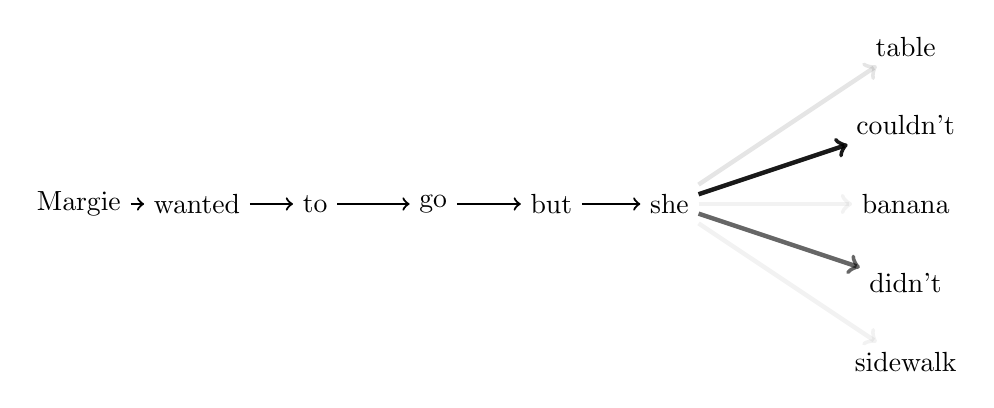
\begin{tikzpicture}[xscale = 1.5]
  \node (W1) at (0, 0) {
    Margie
  };


  \node (W2) at (1, 0) {
    wanted
  };

  \node (W3) at (2, 0) {
    to
  };

  \node (W4) at (3, 0) {
    go
  };

  \node (W5) at (4, 0) {
    but
  };

  \node (W6) at (5, 0) {
    she
  };

  \node (W7) at (7, 2) {
    table
  };

  \node (W8) at (7, 1) {
    couldn't
  };

  \node (W9) at (7, 0) {
    banana
  };

  \node (W10) at (7, -1) {
    didn't
  };

  \node (W11) at (7, -2) {
    sidewalk
  };

  \draw[thick, ->] (W1) -- (W2);
  \draw[thick, ->] (W2) -- (W3);
  \draw[thick, ->] (W3) -- (W4);
  \draw[thick, ->] (W4) -- (W5);
  \draw[thick, ->] (W5) -- (W6);
  \draw[ultra thick, ->, opacity = 0.1] (W6) -- (W7);
  \draw[ultra thick, ->, opacity = 0.9] (W6) -- (W8);
  \draw[ultra thick, ->, opacity = 0.05] (W6) -- (W9);
  \draw[ultra thick, ->, opacity = 0.6] (W6) -- (W10);
  \draw[ultra thick, ->, opacity = 0.05] (W6) -- (W11);
\end{tikzpicture}

    }
  \end{figure}

  \begin{align*}
    P(u) &= \text{softmax}(h_{n}W_{e}^{T})\\
    L_{1}(\mathcal{U}) &= \sum_{i} \text{log} \,P(u_{i} | u_{i - k}, \dots, u_{i - 1}; \Theta)
  \end{align*}

  \begin{description}[leftmargin=!,labelwidth=\widthof{\bfseries Hardware}]
  \item[Dataset] BooksCorpus (7000 books, $\sim$ 800M words, $\sim$ 5GB of text),
  \item[Duration] 1 month,
  \item[Hardware] 8 GPUs.
  \end{description}
\end{frame}
%%%%%%%%%%%%%%%%%%%%%%%%%%%%%%%%%%%%%%%%%%%%%%%%%%%%%%%%%%%%%%%%%%%%%%

%%%%%%%%%%%%%%%%%%%%%%%%%%%%%%%%%%%%%%%%%%%%%%%%%%%%%%%%%%%%%%%%%%%%%%
\begin{frame}
  \frametitle{Supervised fine-tuning}

  \framesubtitle{Multitask learning}

  \fontsize{7.5pt}{7.2}\selectfont

  \begin{figure}
    \begin{tikzpicture}[xscale = 4.5]
  \node (TNFigure) at (0, 0) {
    \includegraphics[width = 2.5cm]{images/openai_transformer.png}
  };

  \node(LMText) at (2, 1) {
    Language modeling loss
  };

  \node(CLFText) at (2, 0) {
    Classification loss
  };

  \node(FText) at (2, -1) {
    Final loss
  };

  \node (LMLoss) at (1, 1){
    $L_{1}(\mathcal{U}) = \sum_{i} \text{log} \,P(u_{i} | u_{i - k}, \dots, u_{u - 1}; \Theta)$
  };

  \node (CLFLoss) at (1, 0){
    $L_{2}(\mathcal{C}) = \sum_{(x, y)} P(y|x^{1}, \dots, x^{m})$
  };

  \node (FLoss) at (1, -1){
    $L_{3}(\mathcal{C}) = L_{2}(\mathcal{C}) + \lambda * L_{1}(\mathcal{C})$
  };
\end{tikzpicture}

  \end{figure}

\end{frame}
%%%%%%%%%%%%%%%%%%%%%%%%%%%%%%%%%%%%%%%%%%%%%%%%%%%%%%%%%%%%%%%%%%%%%%

%%%%%%%%%%%%%%%%%%%%%%%%%%%%%%%%%%%%%%%%%%%%%%%%%%%%%%%%%%%%%%%%%%%%%%
\begin{frame}

  \frametitle{Results on standard datasets}

  New state of the art on the following tasks:

  \bigskip

  \begin{itemize}
  \item Textual Entailment
    \begin{itemize}
      \footnotesize
    \item SNLI $89.3 \rightarrow 89.9$
    \item MNLI Matched $80.6 \rightarrow 82.1$
    \item MNLI Mismatched $80.1 \rightarrow 81.4$
    \item SciTail $83.3 \rightarrow 88.3$
    \item QNLI $82.3 \rightarrow 88.1 $
    \end{itemize}
    \smallskip
  \item Semantic Similarity
    \begin{itemize}
      \footnotesize
    \item STS-B $81.0 \rightarrow 82.0$
    \item QQP $66.1 \rightarrow 70.3$
    \end{itemize}
    \smallskip
  \item Reading Comprehension
    \begin{itemize}
      \footnotesize
    \item RACE $53.3 \rightarrow 59.0$
    \end{itemize}
    \smallskip
  \item Commonsense Reasoning
    \begin{itemize}
      \footnotesize
    \item ROCStories $77.6 \rightarrow 86.5$
    \item COPA $71.2 \rightarrow 78.6$
    \end{itemize}
    \smallskip
  \item Linguistic Acceptability
    \begin{itemize}
      \footnotesize
      \item CoLA $35.0 \rightarrow 45.4$
    \end{itemize}
    \smallskip
  \item Multi-Task Benchmark
    \begin{itemize}
      \footnotesize
      \item GLUE $68.9 \rightarrow 72.8$
    \end{itemize}
  \end{itemize}

\end{frame}
%%%%%%%%%%%%%%%%%%%%%%%%%%%%%%%%%%%%%%%%%%%%%%%%%%%%%%%%%%%%%%%%%%%%%%

%%%%%%%%%%%%%%%%%%%%%%%%%%%%%%%%%%%%%%%%%%%%%%%%%%%%%%%%%%%%%%%%%%%%%%
\begin{frame}
  \frametitle{Input formatting}

  \begin{figure}
    \includegraphics[width = 8cm]{images/input_formatting.png}
  \end{figure}

  Two possible input shape:

  \begin{itemize}
  \item \texttt{(batch\_idx, token\_idx, 2)}
  \item \texttt{(batch\_idx, sequence\_idx, token\_idx, 2)}
  \end{itemize}

  \bigskip

  The \texttt{2} is there to select either the token embedding or its
  corresponding position embedding.
\end{frame}
%%%%%%%%%%%%%%%%%%%%%%%%%%%%%%%%%%%%%%%%%%%%%%%%%%%%%%%%%%%%%%%%%%%%%%

%%%%%%%%%%%%%%%%%%%%%%%%%%%%%%%%%%%%%%%%%%%%%%%%%%%%%%%%%%%%%%%%%%%%%%
\begin{frame}[fragile]
  \frametitle{Input formatting}

  \begin{lstlisting}
def transform_imdb(X, encoder, max_len, n_vocab, n_special,
                   n_ctx):
    n_batch   = len(X)
    xmb       = np.zeros((n_batch, n_ctx, 2), dtype = np.int32)
    mmb       = np.zeros((n_batch, n_ctx), dtype = np.float32)
    start     = encoder['_start_']
    clf_token = encoder['_classify_']
    for i, x in enumerate(X):
        x_with_tokens   = [start] + x[:max_len] + [clf_token]
        l_x             = len(x_with_tokens)
        xmb[i, :l_x, 0] = x_with_tokens
        mmb[i, :l_x]    = 1
    pos_emb_start = n_vocab + n_special
    xmb[:, :, 1]  = np.arange(
        pos_emb_start,
        pos_emb_start + n_ctx
    )

    return xmb, mmb
  \end{lstlisting}
\end{frame}
%%%%%%%%%%%%%%%%%%%%%%%%%%%%%%%%%%%%%%%%%%%%%%%%%%%%%%%%%%%%%%%%%%%%%%

%%%%%%%%%%%%%%%%%%%%%%%%%%%%%%%%%%%%%%%%%%%%%%%%%%%%%%%%%%%%%%%%%%%%%%
\begin{frame}
  \frametitle{BERT: Pre-training of Deep Bidirectional Transformers
    for Language Understanding}

  \begin{figure}
    \includegraphics[width = 8cm]{images/bert.png}
  \end{figure}

  \emph{BERT} is an improvement on the GPT. The main differences are:
  \begin{itemize}
  \item Bidirectional training,
  \item Different pre-training tasks (masked language model and next
    sentence prediction),
  \item Trained on a much bigger corpus (BookCorpus (800M words) \textbf{+
    Wikipedia (2500M words)}),
  \item 3 $\times$ as many parameters for the large version,
  \item Pre-trained model for 102 languages.
  \end{itemize}

  Google's BERT produces 11 new SOTAs on top of the 9 of OpenAI's GPT.
\end{frame}
%%%%%%%%%%%%%%%%%%%%%%%%%%%%%%%%%%%%%%%%%%%%%%%%%%%%%%%%%%%%%%%%%%%%%%

%%%%%%%%%%%%%%%%%%%%%%%%%%%%%%%%%%%%%%%%%%%%%%%%%%%%%%%%%%%%%%%%%%%%%%
\begin{frame}
  \frametitle{References}

  \fontsize{6pt}{7.2}\selectfont

  \begin{itemize}
  \item Tensorflow GPT: \href{https://github.com/openai/finetune-transformer-lm}{https://github.com/openai/finetune-transformer-lm}

  \item Tensorflow BERT: \href{https://github.com/google-research/bert}{https://github.com/google-research/bert}

  \item PyTorch GPT: \href{https://github.com/huggingface/pytorch-openai-transformer-lm}{https://github.com/huggingface/pytorch-openai-transformer-lm}

  \item PyTorch BERT: \href{https://github.com/huggingface/pytorch-pretrained-BERT}{https://github.com/huggingface/pytorch-pretrained-BERT}

  \item IMDB movie review classification: \href{https://github.com/rodgzilla/pytorch-openai-transformer-lm/tree/movie_reviews_classification}{https://github.com/rodgzilla/pytorch-openai-transformer-lm/tree/movie\_reviews\_classification}

  \item Bai, Shaojie, J. Zico Kolter, and Vladlen Koltun. "An
    empirical evaluation of generic convolutional and recurrent
    networks for sequence modeling." arXiv preprint arXiv:1803.01271
    (2018).

  \item Vaswani, Ashish, et al. "Attention is all you need." Advances
    in Neural Information Processing Systems. 2017.

  \item Radford, Alec, et al. "Improving language understanding by generative pre-training." URL
    \href{https://s3-us-west-2.amazonaws.com/openai-assets/research-covers/language-unsupervised/language_understanding_paper.pdf}{Article pdf link}
    \href{https://blog.openai.com/language-unsupervised/}{Blog post} (2018).

  \item Devlin, Jacob, et al. "BERT: Pre-training of Deep
    Bidirectional Transformers for Language Understanding." arXiv
    preprint arXiv:1810.04805 (2018).
  \end{itemize}
\end{frame}
%%%%%%%%%%%%%%%%%%%%%%%%%%%%%%%%%%%%%%%%%%%%%%%%%%%%%%%%%%%%%%%%%%%%%%

\end{document}
